\documentclass{homework}
\title{Homework 4}
\begin{document}
\maketitle

\begin{problem}
By the fact that orthogonal elements must be linearly independent, \(p_0, \dots, p_n\) must span an \((n+1)\)-dimensional linear subspace of the polynomials, and since they are all inside \(\mathbb P_n\), which happens to be \((n+1)\)-dimensional, we showed that they span \(\mathbb P_n\).

Suppose \(p_n\) has repeated roots. Then consider \(u = \prod_k (x-x_k)\), where \(x_k\) are the roots of \(p_n\), but with two repetitions of the roots removed. Then \(p_n(x)u(x)\) is either non-negative, or non-positive, since every root is repeated an even number of times. Also it is not zero, so \(u\) cannot be orthogonal to \(p_n\), because \(w(x) \ge 0\), and
\[(u, p_n)_w = \int_{-1}^1 u(x) p_n(x) w(x) \d[x].\]
(To be rigorous we need some measure theory to guarantee that this integral is not just zero, since \(w\) is only assumed to be integrable.)
On the other hand, \(u\) is in \(\mathbb P_{n-2}\), so it can be expressed as \(\sum{i=0}^{n-2} c_i p_i\). But each of these is orthogonal to \(p_n\), so their sum must also be. This is a contradiction, therefore \(p_n\) cannot have repeated roots.

Suppose \(p_n\) has a root \(\tilde x\) outside of \((-1,1)\), then we consider \(u\) again, but this time \(x_k\) are the roots of \(p_n\) with \(\tilde x\) removed. The exact same logic leads to a contradiction. So no roots can occur outside of \((-1,1)\) either.
\end{problem}

\begin{problem}
From measure theory we know that polynomials are dense in the space of continuous functions (equipped with the supremum norm). Therefore for a continuous function there are a sequence of polynomials \(p_n\) such that
\[\lim_{n\to\infty} \sup_{x \in [a,b]} |f(x) - p_n(x)| = 0.\]
% Without loss of generality we may assume that \(p_n\) has degree at most \(n\), since we can always duplicate the polynomials in the sequence without changing the convergence property, so we can duplicate each polynomial enough times so that \(\deg p_n \le n\) is satisfied. 
Since the quadrature is interpolatory, when \(m \ge \deg p_n\), the \(m\)-th interpolated polynomial of \(p_n\) would be exactly \(p_n\). So we have \[I_m(p_n) = \int_a^b p_n(x) \d[x] \quad (m \ge \deg p_n).\] Therefore we need only establish a bound on \(|I_m(p_n) - I_m(f)|\). Since all the weights are non-negative, we have
\begin{align*}
|I_m(p_n) - I_m(f)|
&= \left| \sum_{k=0}^m \omega_k [p_n(x_k) - f(x_k)] \right|\\
&\le \sum_{k=0}^m \omega_k |p_n(x_k) - f(x_k)|\\
&\le \sum_{k=0}^m \omega_k \overbrace{\sup_{x \in [a,b]} |f(x) - p_n(x)|}^{c_n}\\
&=I_m(c_n) = c_n(b-a).
\end{align*}
The last step is because the interpolation of a constant function (i.e. a zeroth degree polynomial) is always exact, and so the integration must be exact. By the initial assumption, \(c_n \to 0\) as \(n \to \infty\). Therefore for any \(\epsilon > 0\), we can pick \(n\) such that \(c_n < \frac\epsilon{2(b-a)}\). Then we have \(|I_m(p_n) - I_m(f)| \le \frac\epsilon 2\) for \(m \ge \deg p_n\), and also
\[\left|\int_{a}^b f(x) - p_n(x) \d[x]\right|
\le \int_a^b |f(x) - p_n(x)| \d[x]
\le c_n(b-a) < \frac\epsilon{2}.\]
Chaining everything,
\[\left|I_m(f) - I(f) \right|
\le \underbrace{|I_m(f) - I_m(p_n)|}_{< \frac\epsilon2} + \underbrace{|I_m(p_n) - I(p_n)|}_{=0} + \underbrace{|I(p_n) - I(f)|}_{<\frac\epsilon2} < \epsilon.\]
This holds for every \(m \ge \deg p_n\). By the definition of limit, we proved that \(\lim_{m\to\infty}I_m(f) = I(f)\).
\end{problem}

\begin{problem} The Chebyshev polynomials are \(T_n(x) = \cos(n\arccos x)\).
\begin{enumerate}[label=(\roman*)]
\item Directly integrate:
\begin{align*}
\int_{-1}^1 T_n(x) \d[x] &= \int_{-1}^1 \cos (n \arccos x) \d[x]\\
&= \int_{0}^{\pi} - \cos(nt)\sin(t) \d[t]\\
&= \frac12\int_0^\pi \sin[(n-1)t] - \sin[(n+1)t] \d[t]\\
&= \frac12\left[ \frac{\cos[(n+1)t]}{n+1} - \frac{\cos[(n-1)t]}{n-1} \right]_{0}^\pi.
\end{align*}
Substituting and noting that \(\cos(k\pi)\) is zero when \(k\) is odd, and is \((-1)^{k/2}\) when \(k\) is even, we get the desired identity.
\item We want to expand a function into Chebyshev polynomials \(f(x) = \sum_{k=0}^\infty c_k T_k(x)\). Since \(T_n(\cos \theta) = \cos(n \theta)\), this suggests us to do the variable change
\[f(\cos\theta) = \sum_{k=0}^\infty c_k \cos(n\theta).\]
This means that \(c_k\) is the \(k\)-th coefficient of the Fourier transform of \(g(\theta) = f(\cos\theta)\), which is even. We then compute
\[\int_{-1}^1 f(x) \d[x] = \int_{-1}^1 \sum_{k=0}^\infty c_k T_k(x) \d[x] = \sum_{\text{\(k\) even}} \frac{2c_k}{1-k^2}.\]
But do note that fast Fourier transform usually gives the answers in exponential format, i.e. \(\sum c_k e^{ik\pi\theta}\), so it needs to be adjusted.
\begin{matlab}
function val = CCquadrature(f, N)
  samples = arrayfun(f, cos((0:2*N-1) / N * pi));
  coef = fft(samples);
  coef(1) = coef(1)/2;
  val = dot(coef(1:2:N), 2 ./ (1 - (0:2:N-1).^2)) / N;
end
\end{matlab}
We evaluate this on two functions (both are integrated on \([-1,1]\)), \(f_1(x) = \frac1{1+x^2}\) and \(f_2(x) = \exp(x)\csc(x)\). The errors are plotted below against the number of samples taken:
\begin{center}
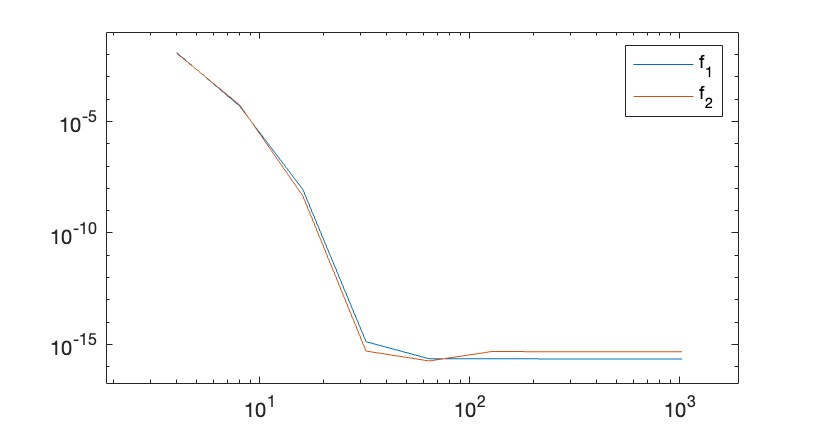
\includegraphics[width=0.7\textwidth]{Hw5-Fig1.jpg}
\end{center}
It is seen that the error quickly reaches machine precision.
\item Obviously we can scale the integrand to work with arbitrary intervals,
\[\int_a^b f(x) \d[x] = \frac{b-a}{2}\int_{-1}^1 f\left(\frac{b-a}{2}x + \frac{b+a}{2}\right) \d[x].\]
But there is also another way. We have
\[\int_a^b f(x) \d[x] = \int_a^b \sum_{k=0}^\infty c_k T_k(x) \d[x].\]
And therefore we only need to recompute the coefficients. Looking back at the integration process in (i), we see that
\[\int T_n(x) \d[x] = \frac12\left[\frac{T_{n+1}(x)}{n+1} - \frac{T_{n-1}(x)}{n-1}\right].\]
In the code we use a lazy way to evaluate Chebyshev polynomials, i.e. by \(T_n(x) = \cos(n\arccos x)\). Since \Matlab\ happens to use complex numbers for \(\arccos\), the result is correct even for \(x \notin [-1,1]\). However, this is effectively trying to Lagrange extrapolate at Chebyshev nodes, which will be pretty bad.

Let's plot \(\int_{-1}^b \frac{\d[x]}{1+x^2}\) using 20 nodes.
\begin{center}
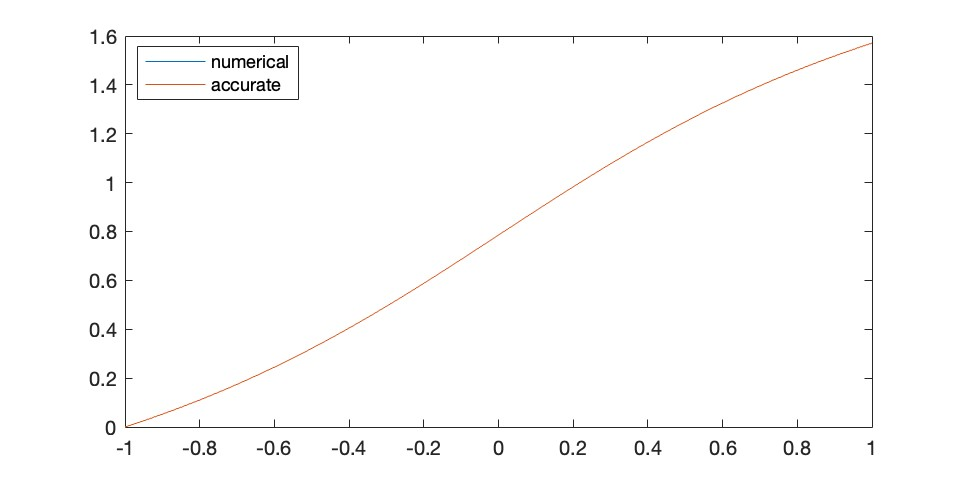
\includegraphics[width=0.7\textwidth]{Hw5-Fig2-1.jpg}
\end{center}

For the next function, let's plot \(\int_{0}^b \sin(10x^2) \d[x]\) with 30 nodes. This time we plot the errors.
\begin{center}
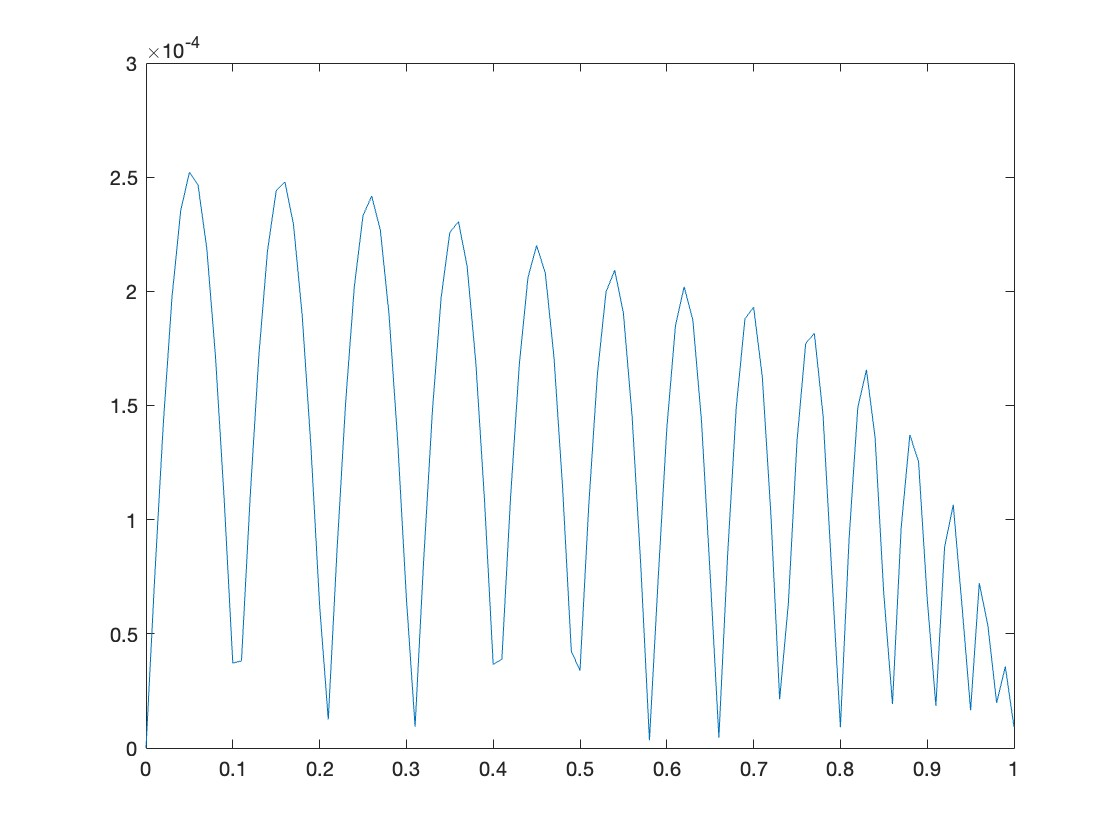
\includegraphics[width=0.7\textwidth]{Hw5-Fig2-2.jpg}
\end{center}
Note how there is the least error around each node. In fact at most of the nodes the error is around machine accuracy. \qed
\end{enumerate}
\renewcommand{\qedsymbol}{}
\end{problem}

\begin{problem}
(i) There isn't too much to explain about the code. The result is as follows:
\begin{center}
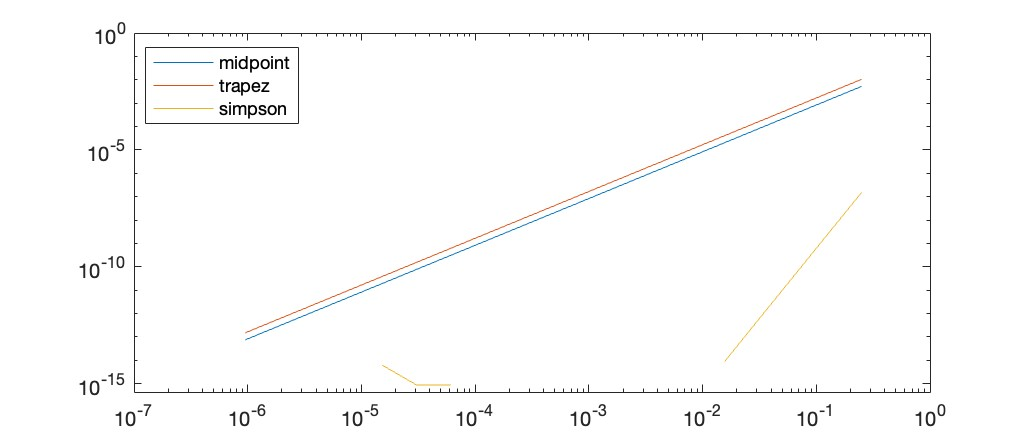
\includegraphics[width=0.7\textwidth]{Hw5-Fig3.jpg}
\end{center}
For the Simpson's rule, the error reaches machine precision at \(h = 2^{-7}\). For the other two, the error is very close to \(Ch^2\), up to the point where smaller \(h\) is not feasible.

(ii) We use Richardson extrapolation on the first ten results of the midpoint rule.
\begin{matlab}
N = 10;
points = integral_midpoint(1:N);
figure(5)
semilogy(abs(points - pi), 'DisplayName', 'R_0');
hold on
for k = (1:N-1)
  points = points(2:N-k+1) + (points(2:N-k+1) - points(1:N-k)) / (4^k - 1);
  semilogy(abs(points - pi), 'DisplayName', 'R_' + string(k));
end
hold off
\end{matlab}
\begin{center}
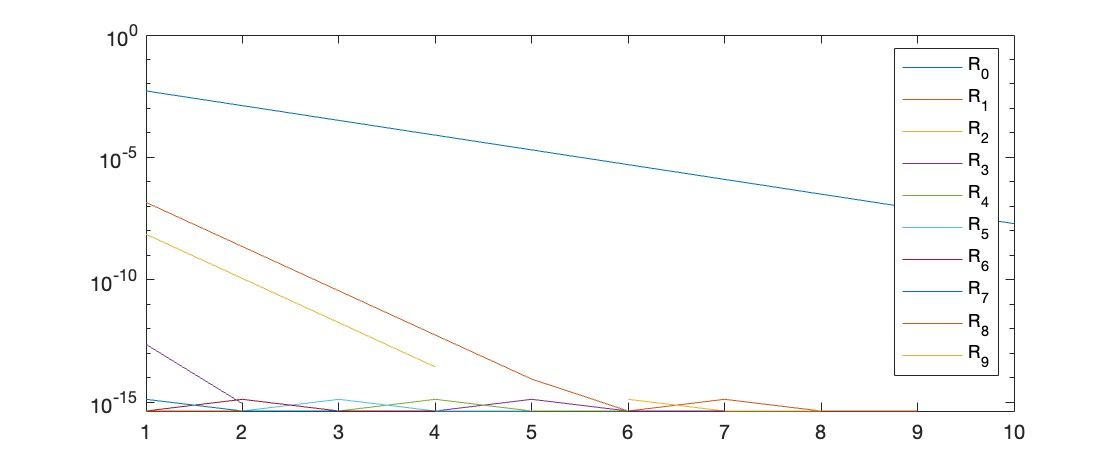
\includegraphics[width=0.7\textwidth]{Hw5-Fig4.jpg}
\end{center}
It is seen that the extrapolation process speeds up the convergence, and very quickly hits machine precision.
\end{problem}

\newpage
\section*{Appendix: Souce Code}
Code can also be found at 
\begin{center}
\texttt{https://github.com/Trebor-Huang/Numerical-Analysis-Homework}
\end{center}
\matlabfile{Hw5.m}

\end{document}
